% !TeX spellcheck = cs_CZ
\wikitextrule
\begin{example}\label{MAI:exam018} 
  Vzorcem $f(x)=\sqrt{1-x}$ je dána funkce, jejímž přirozeným oborem je interval 
  $(-\infty,1\rangle$ (uvažme, že výraz $\sqrt{1-x}$ je definován v reálném oboru, je-li 
  $1-x\geq0$). Graf této funkce je část paraboly, jejíž osou je osa $x$, viz obr. 
  \ref{mai:fig006}.
  
  {\centering
   \captionsetup{type=figure}
%  % !TeX spellcheck = cs_CZ
% mai_fig006.tex

\documentclass[11pt]{standalone}
\usepackage{xltxtra}
\usepackage[usenames,x11names]{xcolor}
\usepackage{tikz}
\usepackage{pgfplots}
  \pgfplotsset{compat=newest}
\usepackage{amsmath}


\begin{document}
  \begin{tikzpicture}[thick,scale=0.7, every node/.style={transform shape}]
    \begin{axis}[
      xmin = -3, xmax = 1.5, ymin = 0, ymax = 3,  % osy
      domain = -3:1,
      restrict y to domain=0:4,
      grid = major,   % both
      grid style={line width=.1pt, draw=gray!20},
      major grid style={dashed, line width=.2pt, draw=gray!40},
      minor tick num=5,
      clip = true,
      clip mode=individual,
      axis x line = middle,
      axis y line = middle,
      xlabel={\(x\)},
    %  xlabel style={at=(current axis.right of origin), anchor=west},
      ylabel={\(y\)},
    %  ylabel style={at=(current axis.above origin), anchor=south},
      enlarge y limits={rel=0.13},
      enlarge x limits={rel=0.07},
    ]
    
     \addplot[color=Gold3, samples=200, smooth, ultra thick, unbounded coords=jump, no markers] 
        gnuplot{sqrt(1-x)};  
    \end{axis}
  \end{tikzpicture}
\end{document} 
   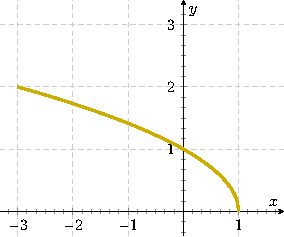
\includegraphics[width=0.5\linewidth]{mai_fig006.pdf}
   \captionof{figure}{{Graf funkce $y=\sqrt{1-x}$ je část paraboly, jejíž hlavní osou je osa $x$}}
   \label{mai:fig006}
   \par}

\end{example}